\documentclass[conference]{IEEEtran}
\IEEEoverridecommandlockouts
\usepackage[T1]{fontenc}
\usepackage{mathptmx}
\usepackage{amsmath,amssymb}
\usepackage{graphicx}
\usepackage{booktabs}
\usepackage[hidelinks]{hyperref}
\title{Coverage or Grouping? Decomposing Ensemble Disagreement to Detect Structural Failures in 3D Fracture Segmentation}
\author{\IEEEauthorblockN{Anonymous authors}}
\begin{document}
\maketitle
\begin{abstract}
Fracture reduction planning requires computed tomography (CT) segmentations in which every bone fragment carries its own label. A model can merge two fragments or split one fragment while predicting almost exactly the right bone surface, so quality-control (QC) signals built on voxel uncertainty or foreground overlap can miss the errors that matter most for planning. We decompose the disagreement between ensemble members into a coverage term, the Jaccard distance between predicted foregrounds, and a grouping term, the variation of information between fragment labelings on the shared foreground, which needs no fragment correspondence. Across 452 controlled interventions in fracture CT, merges and splits changed only the grouping term, whereas fragment removal and boundary shifts changed only the coverage term. The normalization of the grouping term decided its influence on a combined score: its median share rose from 7\% with log-voxel-count normalization to 59\% with joint-entropy normalization. On 200 bones from 100 held-out CT scans, grouping alone ranked merge and split errors with an area under the risk--coverage curve (AURC) of 0.272, against 0.494 for foreground disagreement, 0.636 for voxel entropy and 0.601 for random ranking (lower is better). Joint-entropy normalization reduced the AURC of the combined score by 0.116 and met the primary criterion against both baselines. Separating coverage from grouping turns ensemble disagreement into a specific, label-free signal for instance-level QC of fracture segmentation.
\end{abstract}
\begin{IEEEkeywords}
instance segmentation, uncertainty, quality control, failure detection, fracture CT
\end{IEEEkeywords}

\section{Introduction}
Computer-assisted reduction of pelvic and femoral fractures starts from a three-dimensional model of every bone fragment. Planning software treats each fragment as a rigid body that is repositioned independently, so the CT segmentation has to delineate bone and also give each fragment its own label~\cite{sang2026,pengwin2026}. Deep instance-segmentation pipelines now reach high agreement with expert annotations on public benchmarks~\cite{sang2026}, yet their outputs are still checked slice by slice before they are used. Automated quality control (QC) can shorten this review by ranking cases so that the most suspicious ones are inspected first, provided that its signal tracks the errors that matter for planning.

In fracture segmentation, the most consequential errors are structural. A merge gives two fragments one label and fuses two rigid bodies into one; a split divides one fragment and creates spurious degrees of freedom. Both errors can leave the predicted bone surface almost unchanged. A merged prediction can therefore reach near-perfect Dice with the reference and show little voxel uncertainty, because the error lies in how the foreground is grouped rather than in where it is. QC signals that aggregate voxelwise uncertainty or foreground overlap~\cite{roy2019,mehrtash2020,zenk2025} are insensitive to this failure mode by construction.

Deep ensembles offer a label-free way to expose structural ambiguity: where independently trained models disagree about how bone divides into fragments, at least one of them is likely wrong~\cite{lakshminarayanan2017}. Measuring that disagreement is not straightforward. Fragment IDs are arbitrary, so the members' label maps cannot be compared voxel by voxel; members may predict different numbers of fragments; and differences in where bone is predicted are entangled with differences in how it is grouped. Matching fragments across members, for example by intersection over union (IoU)~\cite{kirillov2019}, needs thresholds and becomes ambiguous precisely when one member merges what another splits.

We separate the two sources of disagreement explicitly (Fig.~\ref{fig:concept}). A coverage term measures foreground disagreement with the Jaccard distance. A grouping term compares the two members' fragment labelings only on voxels that both predict as bone, using the variation of information (VI)~\cite{meila2007}, a distance between partitions that is invariant to label permutation and requires no fragment matching. Combining the two terms raises a design question that turns out to be decisive: the normalization of VI determines whether grouping can influence the combined score at all. This paper makes three contributions:
\begin{enumerate}
\item a coverage/grouping decomposition of ensemble disagreement for fragment-level segmentation, with controlled verification that each term responds only to its intended error mechanism and an analysis of how normalization governs the grouping contribution;
\item a held-out benchmark of 12 prediction-only QC scores on 200 bones from 100 CT scans, in which grouping ranks merge/split errors far better than foreground and entropy baselines and joint-entropy normalization lowers the combined score's AURC by 0.116;
\item an endpoint-level analysis that shows which component aligns with which failure type, giving a principled basis for choosing a QC score according to the review objective.
\end{enumerate}

\begin{figure*}[t]
\centering
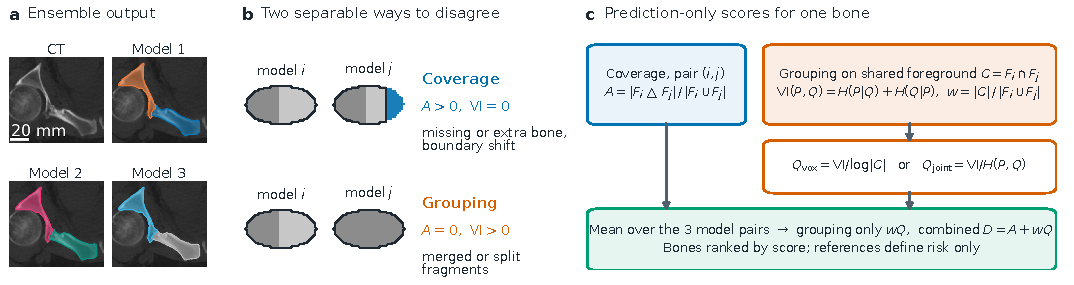
\includegraphics[width=\textwidth]{figures/fig1_concept.pdf}
\caption{Coverage and grouping disagreement on a real fracture CT. (a)~Reference fragment map of a fractured sacrum (PENGWIN 2026 case not used for training or evaluation; coronal slice, three fragments). (b)~Controlled copies of this map and their terms against the reference, computed on the whole 3D bone. Merge and split change only the grouping term; fragment removal and a one-voxel boundary shift (Dice 0.90) change only the coverage term. Dashed outlines mark the merged or removed fragment; white pixels mark the removed rim. For the same VI, log-voxel normalization compresses the grouping term by an order of magnitude ($wQ_{\rm vox}=0.03$ versus $wQ_{\rm joint}=0.40$ for the merge). (c)~Score for one bone from two ensemble members. The heat map is the contingency table of the merge example on the shared voxels $C$ (rows: reference fragments; columns: labels of the copy); VI is computed from these proportions without matching labels. Reference labels enter evaluation only.}
\label{fig:concept}
\end{figure*}

\section{Related Work}
\textit{Segmentation QC.} Ensembles and Monte Carlo sampling provide voxelwise uncertainty~\cite{lakshminarayanan2017,mehrtash2020}, and structure-wise aggregation of this uncertainty supports segmentation QC~\cite{roy2019}. Failure-detection benchmarks have shown that the aggregation step largely determines the value of a confidence signal and that risk--coverage analysis is the appropriate evaluation~\cite{zenk2025,jaeger2023,geifman2017}; pairwise Dice between ensemble members was among the strongest image-level detectors in medical segmentation~\cite{zenk2025}. We include it as a baseline and show that it inherits the blindness of foreground overlap to regrouping. Reverse classification accuracy estimates the quality of a new segmentation from a reference library without a target-case reference~\cite{valindria2017}, and annotation inspection checks labeled training data~\cite{schilling2023}; both are complementary to the prediction-only setting studied here.

\textit{Instance comparison.} Object-level evaluation commonly matches instances by IoU, as in panoptic quality~\cite{kirillov2019}, and instance uncertainty can be derived from matched samples~\cite{siddiqui2024}. Matching introduces thresholds and one-to-one constraints that are ill-defined when one member merges what another splits. We include anatomy-constrained Hungarian matching as a control and compare it with a grouping measure that needs no correspondence.

\textit{Partition comparison.} VI compares partitions independently of their label values~\cite{meila2007}, and its normalized variants differ in how they behave as the number of compared items grows~\cite{vinh2010}. This property matters for 3D bones, whose voxel counts span an order of magnitude. We apply these established measures separately to coverage and to shared-foreground grouping and test their normalization and ranking consequences for fracture QC. Following the principle of problem-aligned validation~\cite{reinke2024,maier2024}, we evaluate every score against several failure definitions.

\section{Methods}
\subsection{Coverage and Grouping Terms}
For one whole 3D bone and two models $(i,j)$, let $F_i,F_j$ be their hard foreground masks, $U=F_i\cup F_j$ the union, and $C=F_i\cap F_j$ the shared foreground. For nonempty $U$, coverage disagreement and shared fraction are
\begin{equation}
A=\frac{|F_i\,\triangle\,F_j|}{|U|},\qquad w=\frac{|C|}{|U|}=1-A ,
\end{equation}
where $\triangle$ denotes symmetric difference. Restricting the two fragment labelings to $C$ defines partitions $P,Q$ of the shared voxels. Their VI is $H(P\mid Q)+H(Q\mid P)$~\cite{meila2007}: each conditional entropy measures the uncertainty that remains about one member's fragment label once the other's is known. Entropies use natural logarithms and the proportions of fragment-label pairs among shared voxels, i.e., the contingency table in Fig.~\ref{fig:concept}c. Because VI depends only on these proportions, it is unchanged by any relabeling of fragments and needs no correspondence between them. It is zero exactly when the two partitions coincide up to relabeling, and positive when one member merges, splits, or redistributes voxels that the other groups differently. Restricting VI to $C$ is what separates the mechanisms: voxels predicted by only one member contribute to $A$ but not to VI, so a missing fragment or a shifted boundary cannot appear as a grouping difference.

We compare log-voxel-count and joint-entropy normalization~\cite{vinh2010}:
\begin{equation}
Q_{\rm vox}=\frac{\mathrm{VI}}{\log|C|},\qquad Q_{\rm joint}=\frac{\mathrm{VI}}{H(P,Q)}\in[0,1],
\end{equation}
where $H(P,Q)$ is the entropy of joint fragment-label pairs on $C$. $Q_{\rm joint}$ depends only on label proportions. $Q_{\rm vox}$ divides by a quantity that grows with bone size and image resolution: across all member pairs in our data, $\log|C|$ ranged from 12.0 to 14.8 (median 12.9), whereas $H(P,Q)$ had medians of 0.29 (development) and 0.26 (held-out) and never exceeded 1.5. The same grouping disagreement is therefore compressed by more than an order of magnitude under $Q_{\rm vox}$, while the coverage term is already a proportion. Weighting grouping by the shared fraction and adding coverage gives
\begin{equation}
D_{\rm vox}=A+wQ_{\rm vox},\qquad D_{\rm joint}=A+wQ_{\rm joint}.
\end{equation}
The weight $w$ discounts grouping evidence that rests on a small shared region. Grouping terms are zero if $|C|\leq1$ or $H(P,Q)=0$; two empty predictions give $A=w=0$, and one empty prediction gives $A=1$. Normalization and weighting occur within each pair, and the resulting scores are averaged over the three member pairs (Fig.~\ref{fig:concept}c). Higher scores give higher review priority. Only predictions enter a score; reference labels are used for evaluation alone.

\subsection{Compared Scores}
All 12 scores in Table~\ref{tab:main} use the same predictions and cover the three families used for segmentation QC. Voxel uncertainty is the mean and 95th-percentile entropy of the ensemble-mean soft foreground probability within the union of hard foreground masks. Foreground overlap is pairwise Dice disagreement and the Jaccard coverage term $A$. Instance-level controls are instance-count variance, VI over the union including background, and anatomy-constrained Hungarian IoU disagreement. The five coverage/grouping scores complete the set. Note that soft foreground entropy and fragment-label entropy describe different distributions: the former quantifies whether a voxel is bone, the latter how bone voxels are grouped.

\subsection{Data and Models}
We used the labeled PENGWIN 2026 Task~1 dataset~\cite{pengwin2026}, which contains pelvic and femoral fracture CT scans with fragment-level annotations. Development comprised 40 CTs and held-out evaluation 100 CTs, both balanced between pelvic and femoral scans and disjoint from training. Held-out cases were sampled with a fixed seed from 210 eligible CTs. Pelvic scans contribute sacrum and left and right hip units, and femoral scans one femur, giving 80 development and 200 held-out bones. A unit is a whole expected 3D bone specified by scan type and is retained even when predictions are empty. Pooled analyses weight bones equally.

The ensemble consisted of three differently seeded members of the pinned, patched two-stage STU-Net implementation~\cite{abbc} built on nnU-Net~\cite{isensee2021}, which performs anatomy localization followed by affinity-based fragment reconstruction. All members used the same 40 training cases. Predicted components below 1{,}000~mm$^3$ were removed with 26-connectivity. Scan metadata and predicted anatomy determine the scoring units. A fourth, separately trained model of the same family provides an independent source of failure labels for a robustness analysis.

\subsection{Failure Endpoints and Statistical Analysis}
The primary structural risk is $(M+S)/\max(N_{\rm ref},1)$, where $N_{\rm ref}$ is the number of reference fragments; it counts merge and split errors per reference fragment and can exceed one. Each reference fragment is assigned to its best-IoU prediction if IoU\,$\geq0.1$. $M$ counts assigned references beyond the first per prediction, and $S$ counts predictions beyond the first overlapping each reference, with any positive overlap qualifying. Risks are computed per model and averaged over the three members.

Two further endpoints describe detection and omission. The original $F_1$ in Table~\ref{tab:main} uses the same best-IoU assignment: precision is the fraction of predictions selected by a reference, recall the fraction of references assigned, and $F_1$ their harmonic mean. Table~\ref{tab:sensitivity}'s one-to-one $F_1$ instead uses maximum-cardinality matching at IoU\,$\geq0.1$. Missing volume is $1-|F_{\rm ref}\cap F_{\rm pred}|/|F_{\rm ref}|$.

QC scores are evaluated as review-ordering rules. For retention coverage $c$, the lowest-scoring fraction $c$ of bones is accepted without review and its mean risk recorded~\cite{geifman2017,jaeger2023}. A useful score accepts error-free bones first, so the retained risk stays low until high coverage. The area under the risk--coverage curve (AURC) summarizes this behavior over all review budgets. It integrates the retained risks at $c=1/n,\ldots,1$, where $n$ is the number of bone units, using trapezoids and expected order within exact ties; lower is better. Paired 10{,}000-resample case-cluster bootstraps are stratified by scan type and carry every bone of each sampled CT; intervals are marginal 95\% CIs. Normalization was chosen on development data. The primary criterion required $D_{\rm joint}$ to improve AURC over both coverage and mean entropy by at least 0.02, with both CIs below zero. Other comparisons are secondary.

\subsection{Controlled Mechanism Tests}
To verify that each term responds only to its intended mechanism, we compared reference instance maps of 20 development CTs (10 per scan type; 40 bones) with controlled copies: unchanged or relabeled; merging one to three nearest fragment pairs; splitting the largest fragment into two to four parts; fragment removal; and boundary shifts to Dice 0.99, 0.95, and 0.90 (tolerance 0.005). Merges that a bone could not support were recorded as ineligible. Separately, all counts of 240 development contingency tables were multiplied by $r\in\{1,2,4,8,16\}$ to test the normalizations at fixed label proportions, i.e., at identical grouping but larger voxel counts.

\begin{figure*}[t]
\centering
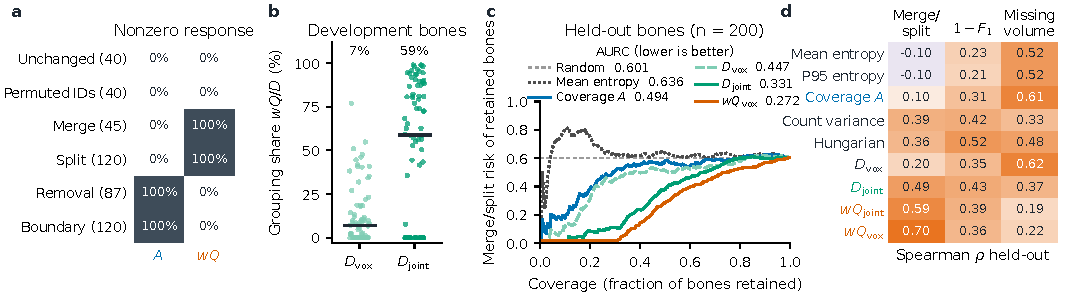
\includegraphics[width=\textwidth]{figures/fig2_evidence.pdf}
\caption{Mechanism, normalization and ranking evidence. (a)~Controlled interventions on reference maps: fraction of eligible interventions (count in parentheses) that produce a nonzero coverage or grouping term. (b)~Share of the grouping term in the combined score for 80 development bones; gray lines connect the same bone, black bars mark medians. (c)~Held-out risk--coverage curves: bones are accepted in order of increasing score, and the curve shows the mean merge/split risk of the accepted bones; legend values are AURC. (d)~Spearman correlation of the same five scores with three failure endpoints on held-out bones (M+S: merge/split risk; Miss.\ vol.: missing volume). All 12 scores appear in Table~\ref{tab:main}.}
\label{fig:evidence}
\end{figure*}

\section{Results}
\subsection{Each Term Responds to Its Own Mechanism}
All 452 eligible interventions produced the expected separation (Fig.~\ref{fig:evidence}a). Every merge (45) and split (120) changed grouping with zero coverage response, and every fragment removal (87) and boundary shift (120) changed coverage with zero grouping response. Unchanged and relabeled maps gave zero for both terms, confirming invariance to fragment IDs. The grouping response was graded: in the four bones eligible at all three merge levels, median $Q_{\rm joint}$ increased from 0.006 to 0.018 to 0.032 as one, two and three fragment pairs were merged. Fig.~\ref{fig:concept}b shows the same behavior on a single sacrum, where a merge leaves the foreground untouched ($A=0$) but yields $wQ_{\rm joint}=0.40$.

\subsection{Normalization Determines the Grouping Contribution}
The grouping term's median share of the combined score increased from 7.0\% under $D_{\rm vox}$ to 58.9\% under $D_{\rm joint}$ (Fig.~\ref{fig:evidence}b). In controlled merges, the median weighted grouping terms were 0.0018 and 0.047, respectively. The count-replication test isolates the cause. Across all 240 tables and all factors $r$, VI, $H(P,Q)$, $A$, $w$, and $Q_{\rm joint}$ were unchanged, whereas $Q_{\rm vox}$ decreased by a median 18\% at $r=16$ among the 154 tables with positive VI. Under $Q_{\rm vox}$, the grouping term thus shrinks as a bone is represented by more voxels, even though its grouping is identical. On 27 of the 80 development bones all members grouped the shared foreground identically, so the increase in share reflects how existing disagreement is normalized rather than a change in the predictions.

\begin{table}[t]
\caption{Bone-level AURC for all 12 scores; lower is better. M+S denotes normalized merge-plus-split risk. Subscripts vox and joint denote normalization by voxel count and joint entropy, respectively. Dev.: 40 development CTs; Eval.: 100 separate evaluation CTs.}
\label{tab:main}
\centering\footnotesize
\setlength{\tabcolsep}{3pt}
\begin{tabular}{lrrr}
\toprule
Score & Dev. M+S & Eval. M+S & Eval. $1-F_1$ \\
\midrule
Mean entropy & 0.6570 & 0.6358 & 0.1757 \\
95th-percentile entropy & 0.6767 & 0.6381 & 0.1784 \\
Foreground Dice disagreement & 0.5442 & 0.4943 & 0.1611 \\
Presence (Jaccard disagreement) & 0.5442 & 0.4942 & 0.1611 \\
Union-normalized VI & 0.4342 & 0.3881 & 0.1534 \\
Instance-count variance & 0.5181 & 0.4704 & 0.1523 \\
Hungarian matching disagreement & 0.3933 & 0.3883 & 0.1331 \\
$D_{\rm vox}$ (combined) & 0.4906 & 0.4472 & 0.1557 \\
$wQ_{\rm vox}$ (partition only) & 0.2706 & 0.2720 & 0.1446 \\
$wQ_{\rm joint}$ (partition only) & 0.2891 & 0.2978 & 0.1424 \\
$D_{\rm joint}$ (combined) & 0.3318 & 0.3311 & 0.1453 \\
$Q_{\rm joint}$ (unweighted VI/H) & 0.2890 & 0.2987 & 0.1414 \\
\bottomrule
\end{tabular}
\end{table}


\subsection{Grouping Prioritizes Held-Out Structural Errors}
Of the 200 held-out bones, 138 had nonzero merge/split risk. Grouping-only scores ranked this endpoint best among the 12 scores, with AURC 0.272 for $wQ_{\rm vox}$ and 0.298 for $wQ_{\rm joint}$ (Table~\ref{tab:main}). Coverage improved on random ranking (0.494 versus 0.601), while mean entropy ranked slightly worse than random (0.636). The curves in Fig.~\ref{fig:evidence}c show where this difference arises. When 30\% of bones are accepted without review, the 60 bones ranked safest by $wQ_{\rm vox}$ contain almost no structural errors (mean 0.013 merge/split errors per reference fragment), whereas those accepted by coverage and entropy carry 0.509 and 0.615, close to the cohort mean of 0.604. Grouping therefore identifies a large set of bones that can be accepted with little risk and concentrates review effort on the remainder.

$D_{\rm joint}$ met the primary criterion. Its AURC differences were $-0.163$ against coverage (95\% CI $[-0.212,-0.117]$) and $-0.305$ against mean entropy ($[-0.372,-0.237]$). Changing only the normalization, from $D_{\rm vox}$ to $D_{\rm joint}$, reduced AURC by 0.116 ($[-0.157,-0.077]$). $D_{\rm joint}$ also improved on the instance-level controls, Hungarian matching ($-0.057$, $[-0.087,-0.030]$) and count variance ($-0.139$, $[-0.182,-0.096]$). Both primary contrasts held when failure labels came from the separately trained fourth model ($-0.128$, $[-0.186,-0.071]$, and $-0.281$, $[-0.351,-0.210]$), so the ranking does not depend on scoring and evaluating with the same three members.

\subsection{Each Component Aligns With a Different Failure Type}
The correlations in Fig.~\ref{fig:evidence}d explain the ordering of the scores. Grouping correlated strongly with structural risk ($\rho=0.70$) and weakly with missing volume ($0.22$); coverage showed the reverse pattern ($0.10$ and $0.61$). Mean entropy correlated with missing volume ($0.52$) but not with structural risk ($-0.10$), consistent with voxel uncertainty concentrating on bone boundaries rather than on fragment grouping. With joint-entropy normalization, the combined score balances the two components ($0.49$, $0.43$ and $0.37$ for the three endpoints), whereas $D_{\rm vox}$ behaves almost like coverage alone.

This alignment determines which score suits which review objective. For the primary merge/split endpoint, grouping alone outperformed the combined score ($D_{\rm joint}-wQ_{\rm vox}=+0.059$, $[0.039,0.080]$). Under the alternative definitions in Table~\ref{tab:sensitivity} (one-to-one $1-F_1$, merge/split counts restricted to overlaps of at least $\tau\in\{0.01,0.1\}$ of the larger object's volume, and missing volume), the two scores performed equivalently: all differences were within $\pm0.008$ and all CIs included zero. The combined score therefore retains the structural ranking of grouping under these definitions while adding sensitivity to omissions. Consistent with the same principle, Hungarian disagreement, which mirrors detection matching, gave the lowest AURC for the detection endpoint $1-F_1$ (0.133; Table~\ref{tab:main}).

\begin{table}[t]
\caption{Supplementary endpoint sensitivity on the same 100 evaluation CTs: joint-entropy combined score minus voxel-normalized partition-only score ($D_{\rm joint}-wQ_{\rm vox}$). Negative AURC differences favor the combined score. Intervals are marginal 95\% paired CT-bootstrap intervals.}
\label{tab:sensitivity}
\centering\footnotesize
\begin{tabular}{lrr}
\toprule
Failure definition & $\Delta$AURC & 95\% CI \\
\midrule
Original M+S & +0.0591 & [+0.0393, +0.0801] \\
One-to-one $1-F_1$ & -0.0016 & [-0.0268, +0.0280] \\
Significant overlap, $\tau=.01$ & +0.0033 & [-0.0079, +0.0143] \\
Significant overlap, $\tau=.10$ & -0.0009 & [-0.0055, +0.0035] \\
Missing volume & +0.0078 & [-0.0138, +0.0357] \\
\bottomrule
\end{tabular}
\end{table}


\begin{figure}[t]
\centering
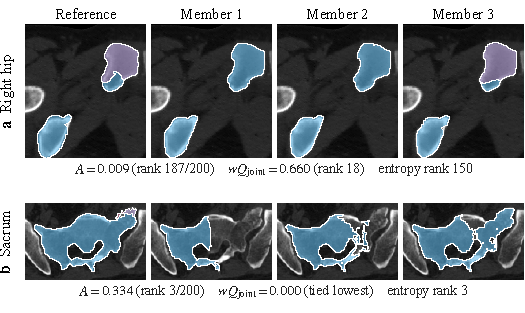
\includegraphics[width=\columnwidth]{figures/fig3_examples.pdf}
\caption{Held-out bones on which the two components diverge (axial slices). Each was selected by a predefined rule among bones with a nonzero error: the largest gap between the flagging component and the other signals (a), or the largest missing volume (b). (a)~Members~1 and~2 assign the displaced fragment the label of the main fragment, whereas member~3 and the reference separate them. The foreground is almost identical across members, so coverage and entropy rank the bone low, but grouping ranks it 18th of 200. (b)~All members group the shared bone identically but omit different parts of the sacrum; coverage ranks the bone third, and grouping is zero. Colors follow the reference fragment with the largest overlap; ranks are among 200 held-out bones (rank~1 = highest review priority).}
\label{fig:examples}
\end{figure}

\subsection{Case Examples}
Fig.~\ref{fig:examples} shows two held-out bones on which the components diverge. In the right hip (Fig.~\ref{fig:examples}a), two members merge a displaced fragment into the main fragment, a structural error that would fuse two rigid bodies in a reduction plan. Because all members cover nearly the same bone, coverage is only 0.009, and coverage and entropy rank the bone 187th and 150th of 200; the grouping term is 0.660 and ranks it 18th, within the first 10\% of the review order. In the sacrum (Fig.~\ref{fig:examples}b), the members agree on how the shared bone is divided but omit different regions, and coverage ranks the bone third of 200. Across the held-out set, four of the six bones with the greatest missing volume had the four highest coverage scores. The two components thus flag different errors, and reporting them side by side also tells the reviewer what kind of error to look for.

\section{Discussion}
Fragment-level QC benefits from measuring coverage and grouping separately. The controlled tests show that the two terms respond to disjoint error mechanisms, and the held-out results show that grouping prioritizes structural errors substantially better than foreground overlap and voxel entropy, the signals most commonly used for segmentation QC. The reason is visible in Fig.~\ref{fig:examples}a: a merge changes how bone is labeled but barely changes where bone is predicted or how confident each voxel is. Independently trained members that resolve an ambiguous fracture line differently produce inconsistent partitions of the same bone, and VI on the shared foreground measures exactly this inconsistency.

The normalization result has a practical lesson for combining heterogeneous disagreement terms. A grouping term normalized by $\log|C|$ shrinks as the number of voxels grows, so for whole 3D bones a combined score silently reduces to its coverage component. Joint-entropy normalization keeps both terms on a proportion scale that does not depend on bone size or image resolution, which is why it lifted the grouping share from 7\% to 59\% and improved the combined score by 0.116 AURC without any change to the predictions.

Our results suggest a simple operating rule. When review targets structural errors, for example before virtual reduction, grouping alone gives the best ordering. When a single score should cover structural errors and omissions, $D_{\rm joint}$ preserves the structural ranking under alternative failure definitions while adding coverage information. In both cases, reporting the two components alongside the score indicates whether a flagged bone is likely to be merged, split or incomplete.

The decomposition is inexpensive to deploy. It is computed from instance label maps that an ensemble already produces, requires no fragment matching, no additional training and no reference annotation, and makes no assumption about the segmentation architecture. The same construction applies in principle to any task in which multiple instances of one structure carry arbitrary labels, such as vertebrae, ribs or teeth, and to other sources of predictions, such as test-time augmentation or Monte Carlo sampling. Reference-library quality estimation~\cite{valindria2017} and expected-anatomy checks are natural complements for errors that all members share.

\section{Conclusion}
Separating coverage from shared-foreground grouping makes ensemble disagreement informative about different fragment-segmentation failures. Controlled tests establish the two responses, joint-entropy normalization lets grouping contribute to a combined score, and held-out evaluation on 200 bones shows that grouping orders structural errors far better than the foreground and entropy signals in current use. Reporting both components together with the target failure definition provides a clear, label-free basis for instance-level QC of fracture segmentation.

\section*{Acknowledgment}
This project is conducted using computational resources from VinUni-Illinois Smart Health Center (VISHC) - VinUniversity. Generative AI tools were used: OpenAI Codex for drafting and manuscript revision. The authors verified all content and take full responsibility for it. The study used public anonymized data; no patients were recruited.

\bibliographystyle{IEEEtran}
\bibliography{references}
\end{document}
